%-----------------------------------------------------------------------------%
% Format and styling in this file originally created by 
% Carl E. Svensson 2010, updated by Adam J. Carmichael 2011
%-----------------------------------------------------------------------------%
%
%- Document Makeup -----------------------------------------------------------%
%- (01) Notes from template author
%- (02) Document Class and Options
%- (03) Standard package includes and options
%- (04) Custom Definitions and Alterations
%- (05) Custom Commands
%- (06) Document title and other metadata
%- (07) Start Document Content
%- (07a) Misc Config
%
%
%- (01) Notes from carneeki@ -------------------------------------------------%
% NEATNESS:
%  Please keep the TeX neat. Best ways to do this:
%  (01) Don't indent
%  (02) Keep inside of 80 characters (it makes for nicer editing on small
%       laptops).
%  (03) Avoid whitespace between \section{} and other document elements. We
%       have %%%% comments for a reason!
%  (04) Use 2 (that's TWO) space characters to indent. NEVER use tab unless
%       your editor converts to to space chars.
%  (05) Maintain customisations in their respective sections.
%  (06) Comment everything. Bandwidth and diskspace are cheap these days, and
%       TeX compresses pretty nice. Anything else is the BAD kind of laziness
%       on your part.
%
% MULTILINE EQUATIONS:
%  Use \begin{align} instead of \begin{eqnarray}...
%  Details as to why are found at (tl;dr : it's just better...):
%  http://texblog.net/latex-archive/maths/eqnarray-align-environment/
% 
% BIBLIOGRAPHY: 
%  -> URLS: to generate the GUID for a reference that is for a URL, paste
%     the URL into goo.gl and then take only the suffix portion.
%
%  -> Wikipedia citations, simply copy + paste the citation from the
%     menu on the LHS.
%
%
%- (02) Document Class and Options -------------------------------------------%
\documentclass[
%  pagesize,
  a4paper,
  pdftex,
%  fontsize=11pt,
  draft=false,
  twoside,
]{book}
%
%
%- (03) Standard package includes and options --------------------------------%
%\usepackage{draftwatermark} % draft watermark. Comment these 2 lines in final
%\SetWatermarkLightness{0.9} %
\usepackage{amsmath}       % amsmath & amssymb are almost ALWAYS required.
\usepackage{amssymb}       %
\usepackage{amsthm}        % for qed, bitches
%
%\usepackage{verbatim}     % multiline commenting ( c++ equiv /* ... */ )
%
\usepackage{xcolor}         % pdflatex
\definecolor{neekiRed}{RGB}{172,40,41}
\definecolor{neekiBlue}{RGB}{62,70,157}
%
\usepackage{geometry}      % option for altering page dimensions if needed
\usepackage[pdftex]{graphicx} % including image files for figures (ie
                              % non-[E]PS)
%                          % valid types: jpeg, png, pdf
\usepackage{wrapfig}       % the figures themselves
\usepackage[numbers,
square,
longnamesfirst
]{natbib}                  % prettybib
\usepackage[pdftex]{hyperref} % clickable TOC and refs
\usepackage[all]{xy}      % category theory helpers
\xyoption{all}            % category theory helpers
\input xy                 % category theory helpers
\usepackage{tikz}        % easy graphic thing
\usetikzlibrary{arrows,shapes,positioning}
\usepackage{tabularx}    % easy tables
\usepackage{url}         % easy urls
\usepackage{multirow}    % 
\usepackage{lipsum}      % autogen placeholder text
%
%- (04) Custom Definitions and Alterations -----------------------------------%
\usepackage[T1]{fontenc} % font-doohickey
%\usepackage{tgadventor}  % font
%\usepackage[math]{iwona} % font
\usepackage[light,math]{kurier} % font
%
\linespread{1.5} % carneeki@ use approx 150% line spacing just like MaxDesign.
\hypersetup{
  % DO NOT CHANGE THESE
%   pdftitle={\metaTitle},
%   pdfauthor={\metaAuthorShort},
%   pdfsubject={\metaSubject},
%   pdfkeywords={\metaKeywords},
  pdfcreator={LaTeX},
  pdfproducer={LaTeX},
  pdftoolbar=false,
  % But change these to taste:
  pdffitwindow=false,   % window fit to page when opened
  pdfstartview={Fit},   % fits the width of the page to the window
                        % all (useful) opts: Fit, FitH, FitV,
  pdfnewwindow=true,    % open links in new window
  colorlinks=true,      % false = boxed links; true = colored links
  linkcolor=neekiRed, % color of internal links
  citecolor=neekiBlue, % color of links to bibliography
  filecolor=red, % color of file links
  urlcolor=red  % color of external links
}
%
%- (05) Custom Commands ------------------------------------------------------%
\newcommand{\derivative}[1][x]{\frac{\mathrm{d}}{\mathrm{d}#1}}
\newcommand{\lxor}{\oplus}
\newcommand{\lxnor}{\lnot\lxor}
\newcommand{\neqref}[1]{\text{(#1)}}
\newcommand{\true}{(\mathbb{T})}
\newcommand{\false}{(\mathbb{F})}
\newcommand{\qedbitches}{\qed}
%
%- (06) Document Title and other metadata ------------------------------------%
%
\title{
  Grokking DMTH137
}
%
\author{
  Adam J. Carmichael \\
  Undergraduate Student \\
  Department of Electronic   Engineering\\
  Macquarie University\\
  Sydney, Australia 2109\\
  Email: \url(adam.carmichael@ieee.org) \\
} % author END Brace
%
%- (07) Start Document Content -----------------------------------------------%
\begin{document}
%- (07a) Misc Config ---------------------------------------------------------%
%-----------------------------------------------------------------------------%
%\cfoot{\thepage\ of \pageref{LastPage}} % page n of m
%
\maketitle
%
%\begin{abstract}
% This document forms the notes for DMTH137 by the author.
%\end{abstract}
%
\section{Introduction}
\label{sec:Introduction}
DMTH137 is about data structures and algorithms.
%-----------------------------------------------------------------------------%
%- Table of Contents ---------------------------------------------------------%
%-----------------------------------------------------------------------------%
\tableofcontents
%
\newpage

%-----------------------------------------------------------------------------%
%- Networks ------------------------------------------------------------------%
%-----------------------------------------------------------------------------%
\chapter{Networks}
\label{chap:Networks}
%-----------------------------------------------------------------------------%
%- Networks :: Undirected and Directed Graphs --------------------------------%
%-----------------------------------------------------------------------------%
\section{Undirected and Directed Graphs}
\label{sec:UndirectedAndDirectedGraphs}

We are used to graphs are often used to describe functions such as $y = f(x)$.
We will not be using them in DMTH137.

It is important to note that a graph is a collection of points
called ``\emph{vertices}'' and lines or connections which join them called
``\emph{edges}''.

A vertex can represent a piece of information and the edge represents how they
are connected.

Example: A vertex represents people and the edges represent the degrees of
separation to which they know eachother.

Example: Each vertex represents a town and the edge represents the distance
between each town.

\emph{Edges must join two distinct vertices}. A graph with loops allows an edge
to join a vertex to itself. (If you have had Cisco switching experience: compare to the
packet storm created in a switched network without spanning tree protocol
implemented).

There are two types of graphs we look at in DMTH137:
\begin{enumerate}
  \item Directed graphs
  \item Undirected graphs
\end{enumerate}

A directed graph has arrows along the edges to indicate the flow of the
direction. Undirected graphs have no arrows. An arrow may point one way, the
opposite way, or double arrows to indicate bidirectionality.

% TODO: include example of directed graph ( ->, <-, <-> )

% TODO: include example of undirected graph 

Sometimes a graph (be it directed or undirected) will have a number or
\emph{weight} with an edge, and is written next to the edge itself.

% TODO: include example of weighted graph.

In terms of language, we say ``Vertex A is adjacent to Vertex B if there is an
edge from A to B''.

\subsection{Equivalence in Graphs}
How do we know when two graphs are the same graph?

When the vertices in one graph, GraphA are able to be translated to a second
graph, GraphB such that both sets of vertices are joined in the same way.

$ A-> (B,C,D) $ % TODO: let this be a messy graph of spaghetti.
$ 1-> (2,3,4) $ % TODO: let this one look like Bruce Schneir's alphabet soup
(through his eyes)

There is only one graph with a single vertex:
% TODO: draw a single vertex
\begin{tikzpicture}
\end{tikzpicture}


2 Vertices:
% TODO: draw 2 points
% TODO: draw 2 points connected

3 vertices:
% TODO: draw 3 points
% TODO: draw 3 points with 2 points connected
% TODO: draw 3 points with 3 points connected

4 vertices:
% TODO: draw 4 points
% TODO: draw 4 points with 2 points connected
% TODO: draw 4 points with 3 points connected 
  % TODO: draw 4 points with 3/4 box
  % TODO: draw 
% TODO: draw 4 points with 4 points connected
  % TODO: draw 4 points as box
  % TODO: draw 4 points with 3/4 box and 1 diagonal

% TODO: just refer to the photos...

Complete graph:

$K_n$ - the complete graph of n vertices is the graph of n vertices
where every pair of vertices is adjacent

$K_3$ (3 points; draw a triangle); 3 edges
$K_4$ (4 points; draw a square and a bend); 5 edges
$K_5$ (5 points; draw a pentagram in a pentagon); 10 edges

Bipartite graph
% TODO: refer to photos
$K_(n,m)$

$K_(3,4)$ (a graph in 2 parts) % bipartite

$K_(3,2)$



%-----------------------------------------------------------------------------%
%- Networks :: Spanning Trees and Traversal Strategies -----------------------%
%-----------------------------------------------------------------------------%
\section{Spanning Trees and Traversal Strategies}
\label{chap:SpanningTreesAndTraversalStrategies}
%-----------------------------------------------------------------------------%
%- Networks :: Walks, Paths and Cycles ---------------------------------------%
%-----------------------------------------------------------------------------%
\section{Walks, Paths and Cycles}
\label{sec:WalksPathsCycles}

An \emph{Eulerian path} is a path in a graph which includes every edge.
An \emph{Eulerian circuit} is an Eulerian path which begins and ends at the same
vertex.

Can an Eulerian path be found on the diagram of ``The 7 Bridges of Konigsber''?

% following diagram courtesy of:
% http://www.texample.net/tikz/examples/bridges-of-konigsberg/
\begin{center}
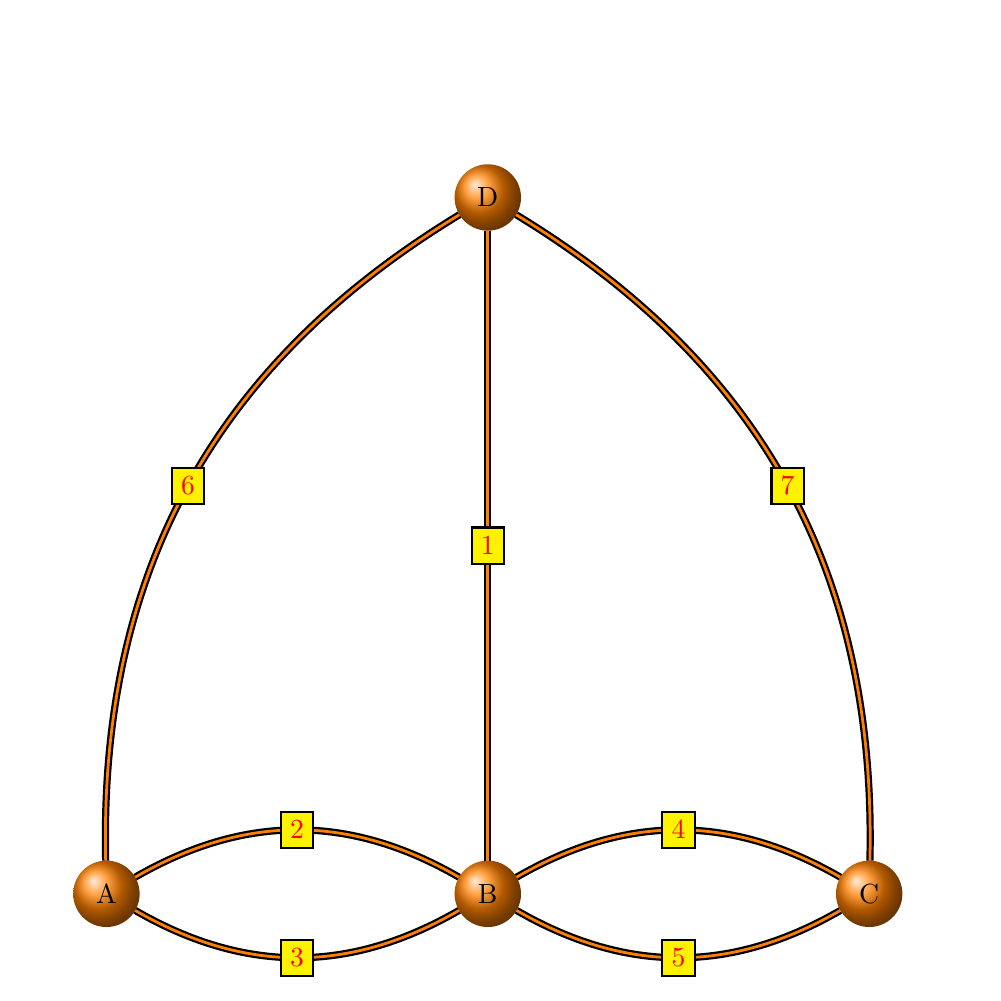
\begin{tikzpicture}[node distance   = 4 cm]
  \useasboundingbox (-1,-1) rectangle (11,11); 
  \tikzset{VertexStyle/.style = {shape          = circle,
                                 ball color     = orange,
                                 text           = black,
                                 inner sep      = 2pt,
                                 outer sep      = 0pt,
                                 minimum size   = 24 pt}}
  \tikzset{EdgeStyle/.style   = {thick,
                                 double          = orange,
                                 double distance = 1pt}}
  \tikzset{LabelStyle/.style =   {draw,
                                  fill           = yellow,
                                  text           = red}}
     \node[VertexStyle](A){A};
     \node[VertexStyle,right=of A](B){B};
     \node[VertexStyle,right=of B](C){C};
     \node[VertexStyle,above= 8 cm of B](D){D};     
     \draw[EdgeStyle](B) to node[LabelStyle]{1} (D) ;
     \tikzset{EdgeStyle/.append style = {bend left}}
     \draw[EdgeStyle](A) to node[LabelStyle]{2} (B);
     \draw[EdgeStyle](B) to node[LabelStyle]{3} (A);
     \draw[EdgeStyle](B) to node[LabelStyle]{4} (C);
     \draw[EdgeStyle](C) to node[LabelStyle]{5} (B);
     \draw[EdgeStyle](A) to node[LabelStyle]{6} (D);
     \draw[EdgeStyle](D) to node[LabelStyle]{7} (C);

  \end{tikzpicture}
\end{center}

\emph{No}. The number of times you enter a circuit equals the number of times
you leave. Each time you enter, you use a different edge. If you enter a vertex
twice, you would have to have used that same entrance twice. Every time you
leave, it is via a different and unused edge.

\section{Minimal Spanning Trees}

A spanning tree in a connected weighted graph with the smallest total weight.

\subsubsection{Kruskal's Algorithm}
Kruskal's algorithm works by using the smallest weight of each edge each time.

First: Create 3 lists:
\begin{enumerate}
  \item All edges in order of increasing weight
  \item edges in tree (initially empty)
  \item current connected components
\end{enumerate}

Remainder of algorithm runs as follows:
\begin{itemize}
  \item Transfer the lowest weight edge from (1) to (2).
  \item Add the vertices at the edge to the appropriate connected component in (3).
  \item Remove from list (1) any edges which join vertices in the same connected component in (3).
  \item Repeat until list (1) is empty.
  \item List (2) contains your minimal tree.
\end{itemize}

% TODO: include photos

\subsubsection{Prim's Algorithm}
Prim's algorithm smoothes over the details by being ``not so greedy''.

3 Lists; similar to Kruskal's lists.
\begin{enumerate}
  \item All edges in order of increasing weight.
  \item edges in tree (initially empty).
  \item Vertices included so far (start with any one vertex).
\end{enumerate}

\begin{itemize}
  \item Transfer the lowest weight edge in list (1) to list (2) which has 1 end
  in list (3) and at the other end of this edge to list (3).
  \item Remove any edge from list (1) which join this new vertex in list(3) to any of other vertices in list(3).
  \item Repeat until list(1) empty.
\end{itemize}

% TODO: include photos

\subsection{Colouring Graphs}
\label{sec:ColouringGraphs}
Colouring graphs so that adjacent vertices have different colours.

Suppose you wanted to draw up the university timetable. We must ensure that no
student is attending two units at the same time.\\
Consider the graph where the vertices are the units and two vertices are joined
if they have a student in common.

% TODO scan in diagram
Can I colour the vertices of this graph such that no two adjacent edges have
the same colour?

(Each colour represent a student, and is also indicative of how many
timetable slots are necessary).


Problem for next week:

Given a graph $G_1$, how many different ways can it be coloured in $K$ colours
so that no two adjacent edges have the same colour?

There is a polynomial that tells us the answer called the \emph{chromatic
polynomial}.

eg (Triangle in TODO). 
$K_3$ using 4 colours.
% Triangle: K=4; use an equilateral triangle

There are 4 different ways to colour the top vertex, 3 different ways to
colour the next, and 2 for the right next after that.
\begin{align}
  4 \times 3 \times 2 & = 24
\end{align}

$K_3$ using 6 colours: 
\begin{align}
  6 \times 5 \times 4 & = 120
\end{align}

$K_3$ using $k$ colours:
\begin{align}
  k \times (k-1) \times (k-2) & = \ldots \\
  & = k^{3} - 3k^{2} + 2k
\end{align}
This is called the \emph{chromatic polynomial for $K_3$}.

% TODO: triangular wheel
$K_4$ using 4 colours:
\begin{align}
  4 \times 3 \times 2 \times 1 & = 24
\end{align}

$K_4$ using $k$ colours:
\begin{align}
  k \times (k-1) \times (k-2) \times (k-3) & = \ldots \\
  & = k^{4} - 6k^{3} + 11k^{2} - 6k
\end{align}
\emph{Chromatic polynomial for $K_4$}

At this point the chromatic polynomial for $n$ vertices with $K_n$ colours:
\begin{align}
  P(k) = k \times (k-1) \times (k-2) \times \ldots \times (k-n+1) & = \ldots
\end{align}

\subsubsection{Unconnected Vertices in a Coloured Graph}
\label{sec:UnconnectedVerticesInAColouredGraph}

% 3 vertices no edges (triangle no lines)
3 vertices no edges (triangle no lines)
\begin{align}
  P(k) = k^{3}
\end{align}

4 vertices:
\begin{align}
  P(k) = k^{4}
\end{align}

$n$ vertices:
\begin{align}
  P(k) = k^{n}
\end{align}

\subsubsection{Trees in Coloured Graphs}
\label{sec:TreesInColouredGraphs}

The chromatic polynomial for any tree on $n$ vertices is
\begin{align}
  k \times (k-1)^{n-1} & = \ldots
\end{align}

Square:

Question: How can I count the number of ways in the case of a square? Just multiplying
won't work because 2 edges will sometimes be
4 3
3 ?

and others

A  B
4  3
2  ?
C  D

Dependent on the different colours chosen.

Answer: We need a clever idea, like, removing an edge:
A  B
+---
|
+---
C  D

This is now a tree, and not the original graph; however, the answer here might help us.
This tree can be coloured in $k(k-1)^{3}$ different ways with $k$ colours.

Colourings where C and D are different are valid colourings for our square. 

For graphs who's C and D have the same colour; will be valid colourings for

% TODO: triangle

These are $k(k-1)(k-2)$.

So
\begin{align}
  P(k) & = k(k-1)^{3} - k(k-1)(k-2) \\
  & = (k-1)(k-1)^{2}k - k((k-2)) \\
  & = \ldots
\end{align}

So for example square:
\begin{align}
  5 \times 4^{3} - 5 \times 4 \times 3
  \intertext{with 5 colours}
  5 \times 64 - 5 \times 12 & = 5 \times \ldots \times 260
\end{align}

\emph{Notion 1:} So far we have the notion that the answer can be determined from a polynomial
we can compute.

\emph{Fact 1:} A graph with $n$ vertices and no edges can be coloured in $k^{n}$
ways.

\emph{Notion 2:} We can reduce the problem of colouring a graph $G$
to a problem involving graphs with fewer edges. \emph{But how?}\\
\\
Consider a graph, $G$ with an edge between vertices A and B (and all sorts of
other edges and vertices). Now consider two graphs formed from $G$, $G_-$ and
$G_=$.\\
\\
$G_-$ is $G$ without the edge AB. \\
$G_=$ is $G$ with edge AB combined into the output (same old edges in it's
output)\\
\\
Notice that a colouring of the graph $G_-$ can either have AB with different
colours, \emph{XOR} AB with the same colour.\\
\\
In first case, we can use the same colouring to colour $G$. In the second case,
edge AB are the same colour, it doesn't matter if A and B are the same colour. \\
\\
This gives rise to \emph{Fact 2:}, the number of ways to colour $G_-$  = 
the number of ways to colour $G$ = the number of ways to colour $G_=$.

\# ways to colour $G$ = \# ways to colour $G_- - $ \# ways to colour $G_=$, or
more mathematically:
\begin{align}
  P_G(k) & = P_{G_-}(k) - P_{G_=}(k)
\end{align}

%G = house
%      A
%    B   C
%    D   E
% now remove ceiling and merge BC into same point:
%
%      A
%      BC
%   D    E
%
% now remove BD
%
%      A
%     BD  C
%         E
%
% now remove CE
%
%      A
%     BD  CE

% Polynomials:
% -> Triangle:
%    $k(k-1)(k-2)$
%    (now factorize)
% -> Tree:
%    $k(k-1)(k-1)(k-1)$
%    (now factorize)


%-----------------------------------------------------------------------------%
%- Networks :: Direct Proofs and Proofs By Contradictions --------------------%
%-----------------------------------------------------------------------------%
\section{Direct Proofs and Proofs by Contradictions}
\label{chap:DirectProofsAndProofsByContradictions}

%-----------------------------------------------------------------------------%
%- Networks :: Number Theory -------------------------------------------------%
%-----------------------------------------------------------------------------%
\section{Number Theory}
Discrete maths concerns itself with 2 main types of numbers:
\begin{enumerate}
  \item Natural numbers, $\mathbb{N}$
  \item Integers, $\mathbb{Z}$
\end{enumerate}

\subsection{Properties of Integers}
\begin{itemize}
  \item $\mathbb{Z}$
  \item Can be added and multiplied. Closure for addition:
  \begin{align}
    a, b \in \mathbb{Z}, \exists c \in \mathbb{Z} \\
    a + b = c
  \end{align}
  \item Associative:
  \begin{align}
    a + (b + c) & = (a + b) + c &
  \end{align}
  \item Special case - $0$.
  \begin{align}
    \exists 0 \in \mathbb{Z}
    a + 0 & = 0 + a & = a
  \end{align}
  
  \item Inverses:
  \begin{align}
    \forall a \in \mathbb{Z} \exists(-a) \in \mathbb{Z}
    \intertext{of}
    a + (-a) & = (-a) + a & = 0
  \end{align}
  
  Theorem: Suppose $b \in \mathbb{Z}$ and $(a+b) = (b+c) = a$ then $b = 0$
  \begin{align}
             b + a & = a \\
      (b+c) + (-a) & = a + (-a) \\
    b + (a + (-a)) & = 0 \\
             b + 0 & = 0 \\
                 b & = a
  \intertext{Alternatively}
                 b & = b + 0 \\
                   & = b + (a+(-a)) \\
                   & = (b + a) + (-a) \\
                   & = a + -(a) \\
                   & = 0 
  \end{align} \qedbitches
  
  \item Multiplication:
  \begin{align}
    \text{closure} && a, b \in \mathbb{Z} \Rightarrow \exists c \in \mathbb{Z} \\
    \text{of} && a \times b & = c \\
    \text{commutativity} && (a \times b) & = (b \times a) \\
    \text{associativity} && (a \times b) \times c & = a \times (b \times c) \\
    \text{Identity}      && \exists 1 \in \mathbb{Z} \text{with propery such that} \\
                         && 1 \times a & = a 
  \end{align}
  
  \item Calculation law:
  \begin{align}
     \text{If} && a, b, c \in \mathbb{Z}; a \neq 0 \\
               && a \times b & = a \times c  \Rightarrow b = c \\
  \text{Then, if} e \in \mathbb{Z} \text{\&} \\
               && e \times a & = a \times e = a \forall a \text{then} \\
               &&          e & = 1 \\
  \text{Proof} && e & = e \times 1 \\
               &&   & = 1
  \end{align}
  \item Distributive law:
  \begin{align}
    a(b+c) & = (ab) + (ac)
  \end{align}
  
\end{itemize}
\subsection{Special subset: Natural Numbers}
$\mathbb{Z}$ has a special subset called the natural numbers, $\mathbb{N}$
with the following properties:
\begin{itemize}
  \item if $a \in \mathbb{Z}$, exactly one of $a \times -a \in \mathbb{N}$
  \item N is closed under addition or multiplication.\footnote{if you add 2
  natural numbers, you get a natural number, if you multiply natural numbers,
  you get a natural number}.
  \item $0$ is in the natural numbers.
  \item
  \begin{align}
    \text{If} S \subseteq \mathbb{N} \text{and} & \\
      & \{ 0 \in S \} \\
      & \{ \text{If} a \in S \} \text{then} a + 1 = S \\
      & \Rightarrow S = \mathbb{N}
   \end{align}
\end{itemize}

\subsection{Divisibility, Prime Numbers, and Common Factors}
\label{sec:DivisibilityPrimeNumbersAndCommonFactors}

\subsubsection{Divisibility}
\label{sec:Divisibility}
We say that ``$a$ divides $b$'' or ``$b$ is divisible by $a$'' if $b$ is a multiple of $a$.
The symbol to represent this we use a vertical bar:
\begin{align}
   a | b   & \text{``a divides b''} \\
   5 ∤ 11  & \text{``5 does not divide 11''} \\
  27 | 0   & \text{``27 divides 0'' \footnote{$\frac{0}{27}$ is actually true, evaluated it is 0}} \\
   0 | 0   & \text{``0 divides 0''} \\
   0 ∤   6
\end{align}

Amongst the natural numbers $\mathbb{N} = \{0, 1, 2, 3, \ldots\}$, 0, 1 are
special. For the others, they are either prime or composite. \\
\emph{Primes} are divisible by exactly 2 numbers, themselves and 1.
\emph{Composittes} are divisible by numbers other than 1 and themselves.
\footnote{1 is neither composite nor prime. It is called \emph{the unit}.}\\
\\
Example:\\
$\{2, 5, 7, 11, 13, 17, 19, 23 \}$ are all prime numers
$\{0,4,6,8,9,10,12,14,15,16,18,20,21,22\}$ are all composite numbers\\

How many prime numbers are there? Infinitely many.

Proof:
\begin{align}
  \text{Suppose there were only finitely many primes:} \\
  S = \{P_1, P_2, P_3, \ldots P_n \} \\
  \text{Consider} \\
  P_1 \times P_2 \times P_3 \ldots \times P_n + 1 & = \ldots \\
   & = \ni S \\
  \text{Is not in S, so it cannot be a prime. So it must have a prime factor.
  But, none of the primes divide it, because they all leave a remainder of 1.
  So it cannot be composite either.} \\
  & \therefore \text{a contradiction.} \\
  & \Rightarrow \text{the set of primes must be infinite.}
\end{align}

The probability of a large number being prime is approximately $\frac{1}{log_n}$.

\subsection{Divisibility}

\subsection{Common Factors \& Greatest Common Factor}
What are the common factors of $28, 164$?

Factors of $28 = \{ 1,2,4,7,14,28 \}$
Factors of $164 = \{1, 2, 4, 41, 82, 164 \}$

The common factors are $\{1,2,4\}$ and the greatest common factor is $4$.

What is the greatest common factor of $1234$ and $5762$?

Doing many divisions is computationally costly and time consuming. We need a
better way to make this computation feasible.\\
\\
By using prime factors (ie factors of a composite number which are prime), we
can determine composite factors much faster:

\begin{align}
  164 & = 2 * 82 \\
      & = 2*2*41 \\
      & = 2^2 * 41 \\
\end{align} 
or
\begin{align}
  2^0 * 41^0 & = 1 \\
  2^1 * 41^0 & = 2 \\
  2^2 * 41^0 & = 4 \\
  2^0 * 41^1 & = 41 \\
  2^1 * 41^1 & = 82 \\
  2^2 * 41^1 & = 164
\end{align}
So $3^2 * 5^3 * 7^4$ has $3*4*5 = 60$ facotrs\\
\\
So factoring both numbers into products of primes will let us find the factors
and common factors easily and so might be a good way to go. 

GCF of $3^2 * 11^4 * 17^3$ is $8! = 1*2*3*4*5*6*7$
is easily worked out:
\begin{align}
  8! & = 2* 3 * 2^2 * 5 * 7 \\
     & = 2^4 * 3^2 * 5 * 7
\end{align}
So the greatest common factor is $3^2 = 9$.

GCF of $2^5 * 3^2 * 11^4 * 17^3$ is $8! = 1*2*3*4*5*6*7$
is easily worked out:
\begin{align}
  8! & = 2* 3 * 2^2 * 5 * *2 * 3* 7 \\
     & = 2^4 * 3^2 * 5 * 7
\end{align}
So the greatest common factor is $2^4 * 3^2 = 9 * 18 = 144$.

However, this is still computationally unfeasable for large numbers as it is
prohibitively time consuming so this method is also impractical, but, the
ancient Greeks knew how to do it easily.

\section{Proof by Induction, Well Ordering and Euclid's Algorithm}
\label{sec:ProofByInductionWellOrderingAndEuclidsAlgorithm}

\quotation{Mathematical induction proves that we can climb as high as we like on
a ladder, by proving that we can climb onto the bottom rung (the basis) and
that from each rung we can climb up to the next one (the induction)}

Question: How can we prove an infinite number of things? ie How can you prove
a formula is always true?

The definition of $\mathbb{N}$ comes to our rescue; it includes the statement:
if $S \in \mathbb{N}$ and $0 \in S$ and $\forall n \in S \Rightarrow (n + 1) \in S $

\subsection{Equivalent ideas to induction}
\label{sec:EquivalentIdeasToInduction}

\subsubsection{Strong induction}
\label{sec:StrongInduction}
Let $S \in \mathbb{Z}$ and suppose that $0 \in S$ and $(forall n \in \mathbb{Z}, (m < n) \Rightarrow n \in S) \Rightarrow n \in S$ \\
\\
Then $S = N$ \\
\\
Example: Prove that every positive integer $> 2$ is the product of primes of 1
or more prime numbers.\\

Let $S = \subseteq \{ \mathbb{N} | n+2$ is the product of 1 or more primes \\
\begin{align}
  0 \in S && \text{Prove zero is in S}\\
  2 = 2 && \\
  \text{Prove n is in S} && \\
  \text{Suppose that} S \in && \\
  \text{I had to debate that} n = S && \\
  \text{Either} n + 2 \text{is a prime} && \\
  \text{or} && \\
  n + 2 && \text{is composite of 2 or more primes} \\
  (n + 2) & = a \times b & \text{where} (0 < a, b < n+1) \\
  && n \leq b < n \\
  \therefore n \in S &&
\end{align}

18 = 2 * 9
   = 2 * 3 * 3 <-- product of primes
17 = cannot be split because\ldots
   = it is already a prime (1 * 17)

\subsubsection{Well Ordering}
\label{sec:WellOrdering}
The well ordering principle states that if $S \subseteq \mathbb{N}$ then
either S is empty or S has a smaller element.

That is to say, every non-empty subset of the natural numbers has a smallest
element.

\begin{align}
  \sum_{r=0}^{n} 4r^{3} & = n^{2}(n+1)^{2} & \\
%  \text{Let C be the set of counter examples - ie prove that C is empty.} && \nonumber \\
%  \text{Suppose C wasn't empty, then \epsilon has a smallest element, S.} && \nonumber \\
%  S \neq 0 \because & \sum_{r=0}^{0} 4r^{2} = 0 = 0^{2} * (0+1) & \\
%  \text{0 isn't in C, so it cannot be the smallest element of C} &&
\end{align}



%-----------------------------------------------------------------------------%
%- Networks :: Modular Arithmetic --------------------------------------------%
%-----------------------------------------------------------------------------%
\section{Modular Arithmetic}
\label{chap:ModularArithmetic}

%-----------------------------------------------------------------------------%
%- The Natural Numbers and Mathematical Induction ----------------------------%
%-----------------------------------------------------------------------------%
\section{The Natural Numbers and Mathematical Induction}
\label{chap:NaturalNumbersAndMathematicalInduction}

%-----------------------------------------------------------------------------%
%- Prime Numbers and Factorisation -------------------------------------------%
%-----------------------------------------------------------------------------%
\section{Prime Numbers and Factorisation}
\label{sec:PrimeNumbersAndFactorisation}

%-----------------------------------------------------------------------------%
%- Greatest Common Divisors and Least Common Multiples -----------------------%
%-----------------------------------------------------------------------------%
\section{Greatest Common Divisors and Least Common Multiples}
\label{sec:GCDandLCM}

%-----------------------------------------------------------------------------%
%- Euclid's Algorithm
%-----------------------------------------------------------------------------%
\section{Euclid's Algorithm}
\label{sec:EuclidsAlgorithm}

%-----------------------------------------------------------------------------%
%- Chinese Remainder Theorem
%-----------------------------------------------------------------------------%

%-----------------------------------------------------------------------------%
%- Logic
%-----------------------------------------------------------------------------%
\chapter{Logic}
\label{chap:Review}

%-----------------------------------------------------------------------------%
%- Logic :: Propositional Logic and Truth Tables
%-----------------------------------------------------------------------------%
\section{Propositional Logic and Truth Tables}
\label{sec:PropositionalLogicAndTruthTables}

A proposition is a statement that is either true or false.

``It is Thursday'' is a statement, which may be true or false depending on the
day.
``Pigs can fly'' is a statement, which is most likely false unless something odd
is done to the pig.
$2 + 3 = 5$ is a statement which turns out to be true (T).
$2 + 3 = 7$ is a statement which turns out to be false (F).
$ -3 < 7  $ (T)
$\frac{5}{4} > \frac{6}{5}$ (T)

Some things which are not propositions:
\begin{itemize}
  \item ``Go away.'' is a statement, but cannot be resolved to a true or false
  value. ``Because it's Monday''. This is only a sentence fragment 
  \item $ x + y $
  \item ``I am lying.'' is a paradox. If you actually are lying, then the
  statement is true and thus no longer a lie (and hence the truth). Paradoxes come about due to
the notion of ``self-reference''.
  \item ``This sentence is false'' is another example. Interestingly though,
  ``This sentence is true'' is not a paradox.
  \item ``Nothing is true'' is another paradox \footnote{and is an oft used
  topic in post-modernism, but that's arts topic and best left to people who
  belong in Y3A}.
  \item Russell's Paradox
\end{itemize}

Most things that we want to say contain more than a single idea so we must
combine, so we must combine propositions in some way.

Propositions are often represented by the letters p and q. They can be combined
using things called ``connectives'' like:
\begin{itemize}
  \item and
  \item or
  \item not
  \item xor
  \item xnor
  \item implies
  \item iff (if and only if)
  \item equivalent
\end{itemize}

Let ``p'' be the statement ``I like tea'' and ``q'' be the statement ``I like
coffee''.

If I wanted to say: ``I like tea and coffee'': $p \land q$
If I wanted to say: ``I like tea or coffee'': $p \lor q$
If I wanted to say: ``I like tea but not coffee'': $p \land \lnot q$
``I don't like tea or coffee'' can be written two ways: $ -(p \lor q)$ or $\lnot p
\land \lnot q $

Let ``p'' be the statement ``It is raining.''
Let ``q'' be the statement ``I need an umbrella.''

If it is raining, then I need an umbrella:

$ p \to q $

ie, the fact that it is raining implies that I need an umbrella.

If it is not raining, so I don't need an umbrella.

$ \lnot p \to \lnot q $

What about $q \to p$?
This says: ``If I need an umbrella, then it is raining.'' This is not
necessarily true as there may be many uses for an umbrella besides keeping rain
off\footnote{eg an umbrella salesman or as a parachute}.

Let ``p'' be the statement ``he is vegetarian''
Let ``q'' be the statement ``he eats no meat''

He is vegetarian if and only if he eats no meat.

$ p \iff q \equiv (p -> q) \land (q -> p)$
This establishes equivalence between proposition p and q.


Conjunction $p \land q$ is true only when both p,q are true.
\begin{table}[!htb]
\label{tab:TruthTableAND}
\begin{tabularx}{\linewidth}{| c | c | X |} \hline
  p & q & $(p \land q)$ \\ \hline \hline
  F & F & F \\ \hline
  F & T & F \\ \hline
  T & F & F \\ \hline
  T & T & T \\ \hline
\end{tabularx}
\caption{Truth Table: logical AND}
\end{table}

Disjunction $p \lor q$ is true when at least one of p,q are true:
\begin{table}[!htb]
\label{tab:TruthTableOR}
\begin{tabularx}{\linewidth}{| c | c | X |} \hline
  p & q & $(p \lor q)$ \\ \hline \hline
  F & F & F \\ \hline
  F & T & T \\ \hline
  T & F & T \\ \hline
  T & T & T \\ \hline
\end{tabularx}
\caption{Truth Table: logical OR}
\end{table}

Negation $\lnot p$ is true when $p$ is false
\begin{table}[!htb]
\label{tab:TruthTableNOT}
\begin{tabularx}{\linewidth}{| c | X |} \hline
  p & $(\lnot p)$ \\ \hline \hline
  F & T \\ \hline
  T & F\\ \hline
\end{tabularx}
\caption{Truth Table: logical NOT}
\end{table}

Conditional $p \to q$ if p then q, or ``p implies q''. This is false when
$p$ is true and $q$ is false with a default condition of true.

\begin{table}[!htb]
\label{tab:TruthTableIMPLIES}
\begin{tabularx}{\linewidth}{| c | c | X |} \hline
  p & q & $(p \to q)$ \\ \hline \hline
  F & F & T \\ \hline
  F & T & T \\ \hline
  T & F & F \\ \hline
  T & T & T \\ \hline
\end{tabularx}
\caption{Truth Table: logical IMPLIES}
\end{table}

A plain English example: It can't rain when there are no clouds, so ``if it is
raining then it is not cloudy'' is false.

Suppose it isn't raining, it could still be cloudy. This remains true.

Converse $q \to p$
\begin{table}[!htb]
\label{tab:TruthTableCONVERSE}
\begin{tabularx}{\linewidth}{| c | c | X |} \hline
  p & q & $(q \to p)$ \\ \hline \hline
  F & F & - \\ \hline
  F & T & - \\ \hline
  T & F & - \\ \hline
  T & T & - \\ \hline
\end{tabularx}
\caption{Truth Table: logical CONVERSE}
\end{table}

If it is cloudy then it is raining (not always true).
q->p is NOT the same as $p -> q$

Contrapositive $\lnot p -> \lnot q$
Use to establish the notion of ``proof by contradiction''.

Double conditional $ p \equiv q $
p if and only if q: p iff q
$p \to q$ and $q \to p$ must both be true
That is $(p \equiv q) \equiv (( p \to q) \land (q \to p))$

\begin{table}[!htb]
\label{tab:TruthTableEQUIVALENCE}
\begin{tabularx}{\linewidth}{| c | c | X |} \hline
  p & q & $( p \equiv q ) \equiv (( p \to q) \land (q \to p))$
                                                    \\ \hline \hline
  F & F & F \\ \hline
  F & T & F \\ \hline
  T & F & F \\ \hline
  T & T & T \\ \hline
\end{tabularx}
\caption{Truth Table: logical DOUBLE CONDITIONAL}
\end{table}

eg let p: 4 is an even number
       q: 4 is divisible by 2
       p and q clearly mean the same thing.
       
Exclusive or (xor) $p \lxor q$
This is true when either p,q is true, but not both.

\begin{table}[!htb]
\label{tab:TruthTableXOR}
\begin{tabularx}{\linewidth}{| c | c | X |} \hline
  p & q & $( p \lxor q )$ \\ \hline \hline
  F & F & F \\ \hline
  F & T & T \\ \hline
  T & F & T \\ \hline
  T & T & F \\ \hline
\end{tabularx}
\caption{Truth Table: logical XOR}
\end{table}

How large should you make your truth table?
\begin{enumerate}
  \item For every variable we have 2 possible values: True and False.
  \item If we have n propositions we need ${2}^{n}$ rows in the truth table.
\end{enumerate}
For example, if we have the variables $p,q,r$ then we need ${2}^{3} = 8$ rows.

% TODO: fix order of operations

Order of operations:

\begin{enumerate}
  \item Do OR connectives
  \item Do AND connectives
\end{enumerate}


Two expressions are logically equivalent if their truth values match for every
combination of the truth values of their atomic propositions\footnote{an atomic
proposition is a proposition cannot be broken down any further}. This is the
same as saying the expressions have the same truth tables.

We want to show $p \land (q \lor r) \equiv ( (p \land q) \lor (p \land r) )$:
\begin{enumerate}
  \item Build truth table. We need 8 rows.
\end{enumerate}

Tautology: In ordinary language it is when you use redundant words which are
unnecessary \footnote{This explanation in itself is a tautology where redundant
and unnecessary mean the same thing}. A tautology is always true. The opposite
of a tautology is a contradiction; which is always false.

Tautology example: $p <-> q $ iff 

\begin{table}[!htb]
\label{tab:TruthTableTautology}
\begin{tabularx}{\linewidth}{| c | c | c | c | X |} \hline
  $p$ & $q$ & $(p \land q) $ & $ \equiv $ & $ (\lnot p \lor \lnot q) $
                                                      \\ \hline \hline
   F  &  F  &               &       &                 \\ \hline
   F  &  F  &               &       &                 \\ \hline
   F  &  F  &               &       &                 \\ \hline
   F  &  F  &               &       &                 \\ \hline
\end{tabularx}
\caption{Truth Table: Tautology}
\end{table}

%-----------------------------------------------------------------------------%
%- Laws of Logic
%-----------------------------------------------------------------------------%
\section{Laws of Logic}
\label{sec:LawsOfLogic}

\begin{align}
  p \land q & 
    & \equiv q \land p
  \label{eq:Commut}
\end{align}

\begin{align}
  p \land (q \land r) &
    & \equiv (p \land q) \land r
  \label{eq:Assoc}
\end{align}

\begin{align}
  p \land p &
    & \equiv p
  \label{eq:Idemp}
\end{align}

\begin{align}
  p \lor p &
    & \equiv p
  \label{eq:Idemp2}
\end{align}

\begin{align}
  p \land (p \lor q) &
    & \equiv p
  \label{eq:Distrib}
\end{align}

\begin{align}
  p \lor (p \land q) & \equiv p
  \label{eq:Distrib2}
\end{align}

\begin{align}
  p \land \mathbb{T} & \equiv p
  \label{eq:IdentAND}
\end{align}

\begin{align}
  p \lor \mathbb{F} & \equiv p
  \label{eq:IdentOR}
\end{align}

\begin{align}
  p \land \mathbb{F} & \equiv F
  \label{eq:Annihil}
\end{align}

\begin{align}
  p \lor \mathbb{T} & \equiv T
  \label{eq:Annihil2}
\end{align}

\begin{align}
  p \land \not p & \equiv \mathbb{F}
  \label{eq:Inv1}
\end{align}

\begin{align}
  p \lor \not p & \equiv \mathbb{T}
  \label{eq:Inv2}
\end{align}

\begin{align}
  -(p \land q) &
    & \equiv -p \lor -q
  \label{eq:deMorgan}
\end{align}

\begin{align}
  -(p \lor q) &
    & \equiv -p \land -q
  \label{eq:deMorgan2}
\end{align}

\begin{align}
  p \to q &
    & \equiv -p \lor q
  \label{eq:Impl}
\end{align}

\begin{align}
  -(-p) &
    & \equiv p
  \label{eq:2Neg}
\end{align}

\begin{align}
  p \leftrightarrow q
    & \equiv (p \to q) \land (q \to p)
  \label{eq:Equiv}
\end{align}
A more complete table of laws can be found on Wikipedia 
%\footnote{
%url{http://en.wikipedia.org/wiki/Propositional_logic#Basic_and_derived_argument_forms}}


% TODO: provide some examples:
Examples:
$ p \land (p \lor q) \equiv p$
  % TODO: this table

Distributive:
$ p \land (q \lor r) \equiv (p \land q) \lor (p \land r)$
  % TODO: this table

De Morgan:
$ -(p \land q) \equiv (-p \lor -q)$
  % TODO: this table
  
Brackets, Negation, OR, AND

Implication:
$ (p \to q) \equiv (-p \lor q)$
\begin{table}[!htb]
\label{tab:TruthTableTautology}
\begin{tabularx}{\linewidth}{| c | c | c | c | c |} \hline
  $p$ & $q$ & $(p \to q)$ & $\equiv$ & $(-p \lor q)$ \\
  0   &   0 &           T &          & \\
  0   &   1 &           F &          & \\
  1   &   0 &           F &          & \\
  1   &   1 &           T &          & \\
\end{tabularx}
\end{table}

We can use the laws of logic to simplify expressions (eg to process a
conditional more efficiently). \\

Example: simplify $(p \to q) \to r$ \\
We know that:
\begin{align}
  (p \to q) \to r
    & \equiv (-p \lor q) \to r       && \neqref{eq:Impl}\\
    & \equiv -(-p \lor q) \lor r     && \neqref{eq:Impl}\\
    & \equiv (-(-p) \land -q) \lor r && \neqref{eq:deMorgan}\\
    & \equiv (p \land -q) \lor r     && \neqref{eq:deMorgan}\\
\end{align}
(recall that L10 = implication)

Simplify $(p \to q) \to p$:
\begin{align}
 (p \to q) \to p
   & \equiv (-p \lor q) \to p       && \neqref{eq:Impl}\\
   & \equiv -(-p \lor q) \lor p     && \neqref{eq:Impl}\\
   & \equiv (-(-p) \land -q) \lor p && \neqref{eq:deMorgan}\\
   & \equiv (p \land -q) \lor p     && \neqref{eq:2Neg}\\
   & \equiv p L4                    && \neqref{eq:IdentAnd}
\end{align}

Simplify $(p \lor -(-p \to q))$:
\begin{align}
  (p \lor -(-p \to q)) & \\
       & \equiv p \lor -(-(-p) \lor q)         && \neqref{eq:Impl}\\
       & \equiv p \lor -(p \lor q)             && \neqref{eq:2Neg}\\
       & \equiv p \lor (-p \land -q)           && \neqref{eq:deMorgan}\\
       & \equiv (p \lor -p) \land (p \lor -q)  && \neqref{eq:Distrib}\\
       & \equiv (\mathbb{T}) \land (p \lor -q) && \neqref{eq:Inverse}\\
       & \equiv (p \lor -q)                     && \neqref{eq:Identity}
\end{align}

By simplifying $p \to (q \to (p \land q)) $:
%\begin{align}
%  p \to (q \to (p \land q))
%    & \equiv -p \lor (q \to (p \land q))      && \neqref{eq:Impl}\\
%    & \equiv -p \lor (-q \lor (p \land q))    && \neqref{eq:Impl}\\
%  \breaktext{something}
%    & \equiv (-p \lor -q) \lor (p \land q)    && \neqref{eq:Assoc}\\
%    & \equiv -(p \land q) \lor (p \land q)    && \neqref{eq:deMorgan}\\
%    & \equiv \mathbb{T}\\
%    & \therefore Tautology
%\end{align}

Show that $(p \lor q) \to r \equiv -r \to -(p \lor q)$:
\begin{align}
  (p \lor q) \to r & \equiv -r \to -(p \lor q) \\
  \intertext{LHS:}
  (p \lor q) \to r & \equiv - (p \lor q) \lor r      && \neqref{eq:Impl}\\
  \intertext{RHS:}
  -r \to -(p \lor q) & \equiv -(-r) \lor -(p \lor q) && \neqref{eq:Impl}\\
    & \equiv r \lor -(p \lor q)                      && \neqref{eq:2Neg}\\
    & \equiv -(p \lor q) \lor r                      && \neqref{eq:Assoc}\\
    & \equiv LHS  
\end{align}

Simplify $ -(p \to (p \lor q)) $:
\begin{align}
  -(p \to (p \lor q)) & \\
  & \equiv -(-p \lor (p \lor q))   && \neqref{eq:Impl}\\
  & \equiv -((-p \lor p) \lor q)   && \neqref{eq:Assoc}\\
  & \equiv -(\mathbb{T} \lor q)    && \neqref{eq:Inverse}\\
  & \equiv -\mathbb{T} && \\
  & \therefore \equiv \mathbb{F} && \\
  & \therefore contradiction
\end{align}

Establish the contrapositive: $ (p \to q ) \equiv (-q \to -p)$
\begin{align}
  \intertext{LHS:}
  p \to q & \equiv -p \lor q         && \neqref{eq:Impl}\\
  \intertext{RHS:}
  -q \to -p & \equiv -(-q) \lor (-p) && \neqref{eq:Impl}\\
            & \equiv q \lor -p       && \neqref{eq:2Neg}\\
            & \equiv -p \lor q       && \neqref{eq:Assoc}
\end{align}

Simplify $p \lor -(p \to -(q \land p))$:
\begin{align}
  p \lor -(p \to -(q \land p)) & \equiv p \lor -(p \to (-q \lor -p))
                                          && \neqref{eq:deMorgan}\\
  & \equiv p \lor -(-p \lor (-q \lor -p)) && \neqref{eq:Impl}\\
  & \equiv p \lor -(-p \lor -q \lor -p )  && \neqref{eq:Assoc}\\
  & \equiv p \lor -(-p \lor -p \lor -q)   && \neqref{eq:Commut}\\
  & \equiv p \lor -(-p \lor -q)           && \neqref{eq:Idempotent}\\
  & \equiv (-(-p) \land -(-q))            && \neqref{eq:deMorgan}\\
  & \equiv p \lor (p \land q)             && \neqref{eq:2Neg}\\
  \therefore & \equiv p                   && \neqref{eq:Absorb}
\end{align}

%-----------------------------------------------------------------------------%
%- Predicate Logic and Negation
%-----------------------------------------------------------------------------%
\section{Predicate Logic and Negation}
\label{sec:PredicateLogicAndNegation}

\subsection{Predicates vs Propositions}
\label{sec:PredicatesVsPropositions}
We want to construct propositions that are either tautologies (always true) xor
contradictions (always false).

Consider the argument:
Let: \\
$p: $ All even numbers are integers\\
$q: $ 8 is even \\
$r: $ 8 is an integer \\
$(p \land q) \to r $
The problem is, this is NOT a tautology. It is inadequate in describing the
argument: \\
``All even numbers are integers and 8 is even, therefore 8 is an integer.''

Consider the argument: \\
``Not all prime numbers are odd, so there is at least one prime that is not
odd.''\\
$p: $ all primes are odd \\
$q: $ there is at least one non-odd prime \\
$-p \to q$ almost describes the argument, but is inadequate as it is not always
true.

To combat the above problems we use \emph{predicate logic}. A predicate is a
statement containing one or more variables. If values are assigned to all the
variables in a predicate the resulting statement is a
proposition.\footnote{Recall: a proposition is something we can decide the truth
value of.}

Example: $x < 5$. This is a predicate. Giving $x$ a value makes it a proposition
such as $x = 3 (\mathbb{T})$ such that $3 < 5 (\mathbb{T})$. \\
Consider the predicate $x < 5 \lor x \leq 5$ which is always true regardless of
the value of x.
We can form a proposition that is always $\mathbb{T}$:\\
For all $x$, $x<5$ or $x \geq 5$. \\
On the other hand \\
For all $x$, $x < 5 \mathbb{F}$.\footnote{If we were to leave out the
words ``for all'', the statement is sometimes true and sometimes false.}\\

There exists an $x$ such that $x < 5 \mathbb{T}$.

``For all'' and ``there exists'' are called \emph{quantifiers}. Two such
quantifiers are:
$\forall =$ ``for all''
$\exists =$ ``there exists''

Every number has a number larger than it.
Every number: $\forall x$
a number larger than x : y
$\forall x, \exists y, y>x$
For all x, there exists y, such that y > x.
% \begin{align}
%   $\forall x, (x < 5) \lor (x \geq 5)$ \\
%   $\forall x, x < 5$ \\
%   $\exists x, x < 5$
%   \intertext{We can shorten (\emph{abstract}) this notation even more:}
%   \text{Let} P(x): x < 5, Q(x): x \geq 5
%   \intertext{Then we can write a), b), c) as:}
%   \text{a)} \forall x, (P(x) \lor Q(x)) \\
%   \text{b)} \forall x, P(x) \\
%   \text{c)} \exists x, P(x) 
% \end{align}

Example: for every number x, there is another number $y$ such that $y = x + 1$.
\begin{align}
  \forall x, \exists y, y = x + 1 (\mathbb{T})
  \intertext{ or }
  \text{Let} P(x,y): y = x + 1 \text{and write} \\
  \forall x \exists y, P(x,y)
\end{align}

Eg there is a number $y$ such that for every number $x$, $y = x + 1$
\begin{align}
  \exists y \forall x, y = x + 1 (\mathbb{F})
\end{align}
These above two examples show that the order in which we write the quantifiers \emph{is important}.

Example: In a system for booking theatre seats, $B(p,s)$ is the predicate ``person $p$ has booked
seat $s$'', which in symbolic form: \\
% \begin{align}
%   \texttext{``seat s has been booked'' :} \\
%     \exists p, B(p,s) \\
%   \text{``person p has booked a seat:''} \\
%     \exists s, B(p,s) \\
%   \text{``All seats are booked:``} \\
%     \forall s, B(p,s) \\
%   \text{``No seat is double booked:`` \\ another way to write this is ``No seat is booked by
%   both person $p$ and person $q$:''} \\
%     \forall s \forall p \forall q ((B(p,s) \lor B(q,s)) \to (p \equiv q))
% \end{align}

Example: ``All swans are black.\footnote{We have some white swans, hence false}'' $\mathbb{F}$
% \begin{align}
%   \text{Let} P(x): $swan s is black$
%   \forall s, P(s) \\
%   \text{Not all swans are black} \\
%   -\forall s, P(s) \equiv \exists s, -P(s) \\
%   \text{ie, there is at least one non-black swan.} 
% \end{align}

Example: ``There is a number $x$ such that $x^{2} = 2$.
\begin{align}
  \text{Let} P(x): x^{2} & = 2 \\
  \exists x, x^{2} & = 2 (\mathbb{T})
\end{align}

``Negation: There is no number who's square is 2.'' We can easily negate it
\begin{align}
  -(\exists x, x^{2} & = 2 )
  \intertext{But we could do better, rewrite as ``ever number doesn't square to 2''}
  \forall x, -(x ^{2} = 2) & \equiv \forall x, x^{2} \neq 2 (\mathbb{F})
\end{align}

\subsection{Negation}
\label{sec:Negation}

Consider the proposition: $\forall x \exists y, y < x$ \\
Negation will \emph{invert}, \emph{reverse}, or \emph{set opposite to} and is denoted by a minus symbol
in these notes. 
\begin{align}
  -(\forall x \exists y, y < x) & \equiv \\
  & \equiv \exists x - (\forall x \exists y, y < x) \\
  & \equiv \exists x \forall y, -(y < x) \\
  & \equiv \exists x \forall y, y \geq x \mathbb{F} 
  \intertext{Which means ``there is a number $x$ that is smaller than every number $y$.'' ($\mathbb{F}$)}\end{align}

Construct the statement: ``Not all prime numbers are odd.'' ($\mathbb{T}$). \\
This means ``There is at least one prime that is not add.'' \\
\begin{align}
  \text{Let} P(x): & \text{``x is a prime number''} \\
  \text{Let} Q(x): & \text{``x is odd''}
  \intertext{To say ``all primes are odd''}
  &  \forall x, P(x) \to Q(x)
  \intertext{To say ``not all primes are odd''}
  & - (\forall x, P(x) \to Q(x) ) \\
  & \equiv \exists x, -P(x) \to Q(x)) \\
  & \equiv \exists x, -(-P(x)) \lor Q(x)) \\
  & \equiv \exists x, (--P(x) \lor -Q(x)) \\
  & \equiv \exists x, (P(x)) \lor -Q(x))
  \intertext{which means: ``There is a number $x$ such that $x$ is prime but $x$ is not odd.'' (T)} 
\end{align}

Example: Negate $\forall x \exists y(y<x) \lor (x$ is odd $)$:
\begin{align}
  -(\forall x \exists y (( y < x) \lor (x \text{is odd}))) & \\
  & \equiv \exists x, -(\exists y (( y < x) \lor (x \text{is odd}))) \\
  & \equiv \exists x \forall y -(( y < x) \lor (x \text{is odd})) \\
  & \equiv \exists x \forall y (-(y<x) \land (x \text{is odd})) \\
  & \equiv \exists x \forall y (-(y<x) \lor -(x \text{is odd})) \\
  & \equiv \exists x \forall y (( y\geq x) \lor (x \text{is even})) \text{($\mathbb{T}$)}
\end{align}

Example: Negate: $\exists x \forall y, (( y=3x) \to (y \geq x))$:
\begin{align}
  (\exists x \forall y, (( y=3x) \to (y \geq x)) ) & \equiv \\
   & \equiv - (\exists x \forall y, (( y=3x) \to (y \geq x))) \\
   & \equiv \exists x -(\forall y, (( y=3x)  \to (y \geq x))) \\
   & \equiv \exists x \forall y, (-((y=3x) \to (y \geq x))) \\
   & \equiv \exists x \forall y, (-(-(y=3x) \lor (y \geq x))) \\
   & \equiv \exists x \forall y, (( -- (=3x) \land -(y \geq x))) \\
   & \equiv \exists x \forall y, ((( y = 3x) \land -(y \geq x))) \\
   & \equiv \exists x \forall y, (( y = 3x)) \land (y<x)) \text{($\mathbb{F}$)}
\end{align}

%-----------------------------------------------------------------------------%
%- Sets: Operation on Sets, Cartesian Products, Power Sets
%-----------------------------------------------------------------------------%
\section{Set Operations, Cartesian Products and Power Sets}
\label{sec:Sets}

``A \emph{set} is a bunch of stuff that we decide to lump together that we identify has some things in common.'' -- Fran Griffin.

A set is denoted by curly braces.

\begin{align}
\intertext{is not a set:}
  1, 2, 3, 4, 5 \\
\intertext{is a set:}
  \{1, 2, 3, 4, 5 \} \\
\end{align}

To say something is in a set:
\begin{align}
  x \in S \\
  \intertext{is an element of S}
\end{align}

To say something is not in a set:
\begin{align}
  x \ni S \\
\end{align}

To say something (T) is a subset of a set (S):
\begin{align}
  T \subset S \\
\end{align}

What is a subset?

Let: A, B be sets, we say  $A \subseteq B$ (A is a \emph{subset} of B) if $\forall x \in A$ we have $x \in B$
ie every element of B is also an element of A

Example:
\begin{align}
  T = \{ 1, 2, 3\}, T \subseteq S \\
  T = \{ 2, 5 \}, T \subseteq S \\
  T = \{ 3 \}, T \subseteq S \\
  T = \{ 1, 2, 4, 7 \}, T \subset S \text{since $ T \ni S $}
\end{align}
Note: $\{3\} \subseteq S $, but $ 4 \in S $

The \emph{empty set} ($\{\} = 0$) is a subset of S:
Note: $\{0\}$ is \emph{not} the empty set, as it has one element of 0.
$0 \in S, S \subseteq S$ \\ 
Note:  $0 \ni S, S \ni S$ \\
(ie, $S \in S$ is allowed, we can get into trouble with Russell's paradox)\\
\\
%[ \ldots [B] ] $ B \subseteq A $

\subsection{Equality of Sets}
\label{sec:EqualityOfSets}
$(A = B) \leftrightarrow (( A \subseteq B) \land (B \subseteq A))$

\emph{Cardinality}: ie size of a set, ie the number of elements

$|A| = $ number of elements of A.\footnote{We use the ``absolute value'' symbols
to determine the cardinality.}

\begin{align}
 |0| = 0 \\
 |S| = 5 \\
\end{align}

Combining Sets:
Let A, B be sets, $A \bigcup B$ is the set containing all the elements of both A and B.
  $x \in A \bigcup B$ if $(( x \in A )) \lor (x \in B))$
eg
\begin{align}
  S = \{ 1,2,3,4,5 \}. T = \{3, 6, 8\} \\
  S \bigcup T = \{1,2,3,4,5,6,9\} \\
\end{align}
Note: expanded elements in a union are listed only once. Order is not important, eg:
\begin{align}
  \{1,2,3\} = \{2, 3, 1\} \\
\end{align}

Definition: Let A, B, be sets $A \bigcap B$ (read as ``A intersect B'') is the set
of elements common to both A and B.\\
\\
$x \in A \bigcap B$ if $(( x \in A) \land (x \in B))$. \\
eg \\
$ S \{1,2,3,4,5\}, T = \{2, 4, 6, 8\}$ \\
$ S \bigcap = \{2, 4\} $ \\
% TODO: venn diagram of A \bigcap B
% TODO: venn diagram of A \bigcup B

$|A \bigcup B | = |A| + |B| - |A \bigcap B|$ \\

\subsection{Universal Set}

$\mathbb{N} = \{ 1, 2, 3, \ldots\} $ Natural Numbers.\footnote{Mathematicians can't decide whether zero is included or not}. \\
$\mathbb{Z} = \{ -3, -2, -1, 0, 1, 2, 3 \} $ Integers. \\
$\mathbb{Q} = \{ \frac{a}{b} | a, b, \in Z, b \neq 0$ Rational Numbers \\
$\mathbb{R} = \{$ numbers that can be written as decimals $\}$. Real numbers. \\

$\pi$, $\emph{e}$, etc\ldots are not rational, but are real.

$\mathbb{N} \subseteq \mathbb{Z} \subseteq \mathbb{Q} \subseteq \mathbb{R} $ \\

$|\mathbb{N}| = \infty$
$|\mathbb{Z}| = \infty$
$|\mathbb{Q}| = \infty$
$|\mathbb{R}| = \infty$

$|\mathbb{N}| = |\mathbb{Z}| = |\mathbb{Q}| < |\mathbb{R}|$ \\
We can list the elements of $\mathbb{N}$ without missing any, 1, 2, 3, \ldots \\
We can list the elements of $\mathbb{Z}$ in correspondance with elements of $\mathbb{N}:$

% TODO: TeXorize this table:
%
% N: 1, 2,  3,  4,  5,  6,  7,  8,   9,  10, 11
% Z: 0, 1, -1,  2, -2,  3, -3,  4,  -4,   5, -5
%

So the sizes of $\mathbb{N}$ and $\mathbb{Z}$ are the same. We can do this same for $\mathbb{Q}$
(as an exercise). We cannot list the elements of $\mathbb{R}$ in correspondance with $\mathbb{N}$.

To see this, suppose we have a list of all real numbers ($\mathbb{R}$):
(where a, b, c, d, e, \ldots are decimal digits)
%0 . a_1 b_1 c_1 d_1 e_1 \\ 
%0 . a_2 b_2 c_2 d_2 e_2 \\
%0 . a_3 b_3 c_3 d_3 e_3 \\
%0 . a_4 b_4 c_4 d_4 e_4 \\
%0 . a_5 b_5 c_5 d_5 e_5 \\
% TODO: vertical 3dots
But if we take one digit from each number in our list and change it then we have:
%0. a_1^1 b_2^1 c_3^1 d_4^1 e_5^1

Which differs form the $i^{th}$ number in my list at the $i^{th}$ digit. Hence, this
number was not in the list.

$|\mathbb{N}| = |\mathbb{Z}| = |\mathbb{Q}|$ is called \emph{``countable
infinity''}. $|R|$ is \emph{``uncountable infinity''}.

Universal Set $\epsilon$: \\
Let $\epsilon = \mathbb{N}$ \\
Let $S = \{1,2,3,4,5\}$ \\
The complement of S:
%TODO: S-bar
$ -S = \{ x \in \mathbb{N} | x \ni S \} $

%TODO: venn diagram of epsilon and S-bar

$S = \{1,2,3,4,5\}$, $T = \{1,2\}$ \\
$S \ T=\{3, 4, 5\}$ or $S - T = \{3, 4, 5 \}$ is read as ``complement of T is S'' \\
$|S - T| = |S| - |S \bigcap T|$ \\
eg \\
$A = \{ x \subseteq \mathbb{Z} | x \geq 5 \}, B \{ x \subseteq \mathbb{Z} | x < 8 $
$|A| = |B| = \infty$
$|A \bigcap B | \{ x \subseteq \mathbb{Z} | (x \geq 5) \land (x < 8)\} = \{5,6,7\} $ 


%-----------------------------------------------------------------------------%
%- Relations: Symmetry, Reflexivity, Transitivity, Equivalence
%-----------------------------------------------------------------------------%
\section{Relations: Symmetry, Reflexivity, Transitivity, Equivalence}
\label{sec:Relations}

%-----------------------------------------------------------------------------%
%- Functions: Injectivity, Surjectivity, Invertibility
%-----------------------------------------------------------------------------%
\section{Functions: Injectivity, Surjectivity, Invertibility}
\label{sec:Functions}

If we have $f:A \to B$ \\
Where \\
$A:$ represents the domain (input set) and \\
$B:$ represents the co-domain (contains out) \\
The range $f \subseteq B$ is the actual output. \\
\\
Everything in A \emph{must} be connected to everything in B.\\
\\
Example: suppose $A = \{1, 2, 3\}$ and $B = \{p,q\}$. \\
\begin{align}
  f & : A \to B \nonumber \\
  f(1) & = p \nonumber \\
  f(2) & = q \nonumber \\
  f(3) & = q \nonumber \\
\end{align}
We say the domain of $f$ is $\{1, 2, 3\}$, the co-domain $f=\{p,q\}$. range $f=\{p,q\}=B$.
This function is a little bit special because the codomain and the range are the same, but
this may not happen all the time.\\
\\
Example, suppose $A = \{1, 2, 3\}$, $B = \{a, b, \ldots, z\}$. \\
\begin{align}
  f & : A \to B \nonumber \\
  f(1) & = q \nonumber \\
  f(2) & = c \nonumber \\
  f(3) & = k \nonumber \\
\end{align}
Domain $f = \{1, 2, 3\} = A$, codomain $f = B = \{a,b,\ldots,z\}$, the range is only
$f = \{c, k, q\} \subseteq B$.\footnote{Sometimes the range is also called the \emph{image}.} \\
\\
Sometimes we say \emph{image f} to mean \emph{range f}: \\
range f = im f = $\{y \in B | f(x) = y$, for some $x \in A\} \subseteq B$. \\
\\
%TODO: right align the following comment
TODO in comments.\\
%$f: \mathbb{Z} \to {0,1}, f(x) = 0$ % 0 if x is even
%                                    % 1 if x is odd
\begin{align}
  f: \mathbb{Z} \to {0,1}, f(x) =
    \left\{
      \begin{array}{l l}
        0 & \quad \text{if $x$ is even} \\
        1 & \quad \text{if $x$ is odd} \\
      \end{array}
    \right.
\end{align}
\\
(This is sometimes called $f(x) = x$ mod $2$.)\\
\\
Domain $f = \mathbb{Z}$, codomain $f = \{0,1\}$, range $f = \{0,1\}$.\\
\\
The functions $f: A\ to B$, $g: A \to B$ are equal iff $f(x) = g(x) \forall x \in A$.\\
\\
%TODO: xypic the following
\\
% .  ==> a      . ==> a
% .  ==> b      . ==> b
% .  ==> c      . ==> c
% A      B      A     C
\\
They might look the same, but they are NOT the same because they have different codomains.
(See xypic in TODO).
\\
Another example: \\
\\
$f:$ DMTH137 $\to$ X5B.T1 \\
\\
$f(p) = s$, when $p \in $ DMTH137 is a student. \\
$s \in $ X5B.T1 is a seat. \\
\\
domain $f = \{$DMTH137 Students $\}$. \\
codomain $f = \{$seats in X5B.T1 $\}$. \\
range $f = \{$ occupied seats $\}$. \\

-----
$\phi : \mathbb{R} \to \mathbb{R}$, $\phi(x) = x^2$ \footnote{$\phi$ is greek letter phi} \\
$\phi(0) = 1$, $\phi(1) = 4$, $\phi(3) = 9$, $\phi(4) = 16$ \ldots \\

% TODO graph y = x^2
TODO: diagram \\
----- \\
What about $\psi: \mathbb{R}^{+} \to \mathbb{R}$ \footnote{$\psi$ is greek letter psi}.
\begin{align}
  \psi(x) & = \sqrt{x} && \mathbb{R}^{+} = \{x \in \mathbb{R} | x > 0 \} \nonumber \\
  \psi(1) & = \pm 1 \
  \psi(4) & = \pm 2 \
  \psi(9) & = \pm 3 \
\end{align}
This is not a function since we have 2 outputs for each input:

% TODO diagram, y = x ^2 (but rotated cw 90 deg)
TODO: diagram \\
We can make this into a function by taking only the positive square root, or only the negative square root. \\
----- \\
Suppose $|A| = n, |B| = m$, how many functions are there from A to B?
\begin{align}
  \text{Let } \{a_1, a_2, a_3, \ldots , a_n\} then \nonumber \
  f(a_1) & \text{has m possible values} \nonumber \
  f(a_2) & \text{has m possible values} \nonumber \
  f(a_3) & \text{has m possible values} \nonumber \
  \ldots \nonumber \
  f(a_n) & \text{has m possible values} \nonumber \
\end{align}
So there are $m \times m \times m \times \ldots \times m = m^n = |B|^{|A|}$ possible
functions from A to B. \\
Eg: $|A|=5, |B| = 3$,  \# $f: A \to B = 3^5 = 243$

\subsection{Properties of functions}
\subsubsection{Injectivity}
Definition: a function $f: A\ to B$ is \emph{one-to-one} or \emph{injective} iff
$f(x_1) = f(x_2) \to x_1 = x_2$ (or, the y-values are unique) \\
\\
Example: \\
Consider $f:$ DMTH137 $\to$ X5B.T1. \\
f is one-to-one, otherwise people are sitting in the same seat.\footnote{which
may or may not be desirable depening on you like your seating} \\
\\
Example: \\
Consider $f: \mathbb{N} \to \mathbb{N}$, $f(x) = 2x$. \\
is $f$ one-to-one? \\
Suppose $f(x_1) = f(x_2)$, then $2x_1 = 2x_2$ so $x_1 = x_2$ hence $f$ is one-to-one. \\
 \\
Example: \\
Consider $f: \mathbb{Z} \to \{0,1\}$. $f(x) = 0$ if x is even, $f(x) = 1$ if x is odd \\

$f$ is not one-to-one $\because f(1) = f(x) = 1$ and $f(2) = f(4) = 0\ldots$ etc \\
\\
We have an infinite domain, but a finite codomain, so f cannot be 1-1. \\
\\
Example: \\
Consider $f: \mathbb{R} \to \mathbb{R}$, $f(x) = x^2$ \\
\\
Suppose $f(x_1) = f(x_2)$ then $x_1^{2} = x_2^{2}$ \\
$x_1^2 - x_2^2 = 0$ \\
$(x_1 - x_2)(x_1 + x_2) = 0$ so $x_1 = x_2 or x_1 = -x_2$ \\
hence $f$ is not one-to-one. \\

\subsubsection{Surjectivity}
A function $f: A \to B $ is \emph{onto} or \emph{surjective} if $\forall y \in B, \exists x \in A$
such that $y = f(x)$ \footnote{ie range f = codomain f}

% TODO: xypic this
%  .    == >  .
%  .    == >  .
%  .    == >  .
%             .
%  A          B
TODO: diagram \\
Example: $f(x) = 0$ if x is even, $=1$ if odd, $f: \mathbb{Z} \to \{0,1\}$. \\
\\
The range of $f = \{0,1\} = $ codomain $f$ \\
$\therefore$ f is surjective. \\
\\
Example: $f:$DMTH137 $\to$ X5B.T1 \\
Not surjective since there are empty seats \footnote{Fran had a sad face when she said this.}
\begin{align}
  f: A \to B \text{is onto if} \forall y \in B \\
  \exists x \in A \text{such that} y = f(x) \\
  \text{range = codomain}
\end{align}
The easiest way to decide if something is surjective is to consider the range.
Example:
\begin{align}
  f: \mathbb{R} \to \mathbb{R}, f(x) = x^2 \\
  \text{range} f = \{ y \in \mathbb{R} | y \geq 0 \} \\
  \text{but codomain} f = \mathbb{R} \\
  \therefore f \text{is not surjective}
\end{align}
On the other hand, $g: \mathbb{R} \to \{x \in \mathbb{R} | x \geq 0 \}$ then $g(x) = x^2$
is surjective. Here we have chosen the codomain to be exactly the range (image) of $f$.

\begin{align}
  f: \mathbb{Z}, f(x) = x^2 \\
  f \text{is not surjective} \because \text{range $7 \in \mathbb{N}$ but there is no $x \in \mathbb{Z}$ such that $f(x) = 7$}
\end{align}

\subsubsection{Invertive Functions}
A function $f: A \to B$ is \emph{invertible} if it is \emph{both one-to-one and
surjective}. In this case, we can define an inverse function:
\begin{align}
  f^{-1} : B \to A \text{such that} x = f^{-1} = y \\
  \forall x \in A, y \subseteq B
\end{align}

%      f ==>
%  .  <===>   .
%  .  <===>   .
%  .  <===>   .
%     <== f^{-1}
%  A          B

Observe that for an invertable function $f: A \to B$ if is surjective so range $f = $ codomain $f = B$.
$x \forall y \subseteq B \exists x \in A$ with $y = f(x)$
$f$ is one-to-one, so each such $x$ is unique, ie $y = f(x)$ has a unique solution. As this is
true $\forall y \subseteq B$ then we can always find $x$ such that $y = f(x)$ \\
ie $f^{-1}$ exists.\\
\\
Example:\\
Consider $f: \mathbb{N} \to \mathbb{N}, f(x) = x$

% TODO:
% Linear graph - y = x, but only the data points from 0 to 5
See TODO:
\\
Is $f$ invertable?: \\
Is $f$ one-to-one? $f(x_1) = f(x_2) \to x_1 = x_2 \therefore$ yes. \\
Is $f$ surjective? range $f = \mathbb{N}$ Yes. \\
\\
Because $f$ is surjective and one-to-one, it is invertable.\\
\\
\\
Example: \\
Consider: $g: \mathbb{N} \to \mathbb{Z}, g(x) = x$ \\
Is $g$ is one-to-one? Yes.
Range $g = \{y \in \mathbb{Z} | y \geq 0\} = \mathbb{N}$
So $g$ is not surjective. Hence $g$ is not invertable.
\\
\\
Example:\\
Let $A = \{1,2,3,4\} = B$ \\
$f: A \to B$ \\ 
$1 \to 3$ one-to-one
$2 \to 1$ surjective since range f=3
$3 \to 4$ hence f is invertable
$4 \to 2$

$f^{-1}: B \to A$ \\
$1 \to 2$
$2 \to 4$
$3 \to 1$
$4 \to 3$

Analogy to SQL, consider the table: \\
\begin{table}[!htb]
\begin{tabularx}{\linewidth}{| c c c c c c c c c c |}
\hline
  SID      & Name    & A1 & A2 & A3 & A4 & A5 & T1 & T2 & Q \\
\hline
  41963539 & Adam    &  4 &  5 &  - &  - &  - &  - &  - & - \\
  12345678 & Michael &  5 &  4 &  - &  - &  - &  - &  - & - \\
  87654321 & Gareth  &  4 &  5 &  - &  - &  - &  - &  - & - \\
  93536914 & Tor     &  5 &  4 &  - &  - &  - &  - &  - & - \\
\hline
\end{tabularx}
\end{table}
``SELECT SID FROM DMTH137;'' \\
Represents a function on the database.\\
Let $Q:A \to B,  A = \{SID\}, B=\{A1\}$
Define $Q$ as ``SELECT SID FROM DMTH137 WHERE A1 = 5;'' \\
$B = \{0,1,2,3,3,4,5\}$ \\
$Q$ is not one-to-one, but is probably surjective as long as someone got each
of these marks. \\
\\
Suppose now we wanted to store the student data. The domain is the SID, and
the codomain is amount of space allocated to storing the data.\\

\subsubsection{}
Number of functions $f: A \to B$ is $|B|^{|A|}$. Now suppose that A and B are
finite sets.\footnote{The vertical bars represent the cardinality of the set}.\\
\\
Number of one-to-one functions:
\begin{align}
  \text{Let} |A| = m, |B| = n \\
  m > n \text{none}
  m \leq n \left\{
    \begin{array}{l l}
      \text{n choices for} & \quad f(x_1) \\
      \text{n-1 choices for} & \quad f(x_2) \\
      \text{n-2 choices for} & \quad f(x_3) \\
      \ldots
      \text{n-m choices for} & \quad f(x_m) \\
    \end{array}
    \right. \\
  n(n-1)(n-2)\ldots(n-m) = \frac{n!}{(n-m)!}
\end{align}

So the number of surjective functions:
\begin{align}
  m & < n: \text{none} & \\
  m & \geq n: \sum_{i=0}^{n}(-1)^{i}(n-i)^{n}(n-i)^{m} & \text{will be done later}
\end{align}

Number of invertable functions:
\begin{align}
  \text{We need a one-to-one} & (m \leq n )\\
  \text{and} & \nonumber \\
  \text{surjective} & (m \geq n) \\
\end{align}
The number of functions is the same as the number of ways of arranging $n$ objects
(elements)\footnote{this is called a \emph{permutation}}.

n choices for first element
n-1 choices for 2nd element
n-2 choices for 3rd element
\ldots
$n(n-1)(n-2)\ldots(2)(1) = n!$
n! invertable functions.

\subsubsection{Infinite sets}
For functions on infinite sets, we can still consider cardinality.

\begin{align}
  \# f: A \to B, = |B|^{|A|} \\
  f: \mathbb{Z} \to \mathbb{N} &
   & f(0) = 0 \\
   & f(1) = 1 \\
   & f(-1) = 2 \\
   & f(2) = 3 \\
   & f(-2) = 4 \\
   & \ldots
\end{align}

We can list all of $\mathbb{Z}$ in one-to-one correspondance with $\mathbb{N}$.
This means that $|\mathbb{Z}| = |\mathbb{N}|$. We can do the same sort of thing
to shoq that $|\mathbb{Q}| = |\mathbb{N}|$. We can't find a function for
$g: \mathbb{R} \to \mathbb{N}$ that is one-to-one and surjective, so
$|\mathbb{R}| \neq |\mathbb{N}|$.

\subsubsection{Composition of Functions}
Suppose $f: A \to B, g: B \to C$. \\
\begin{align}
  \text{Let} x \subseteq A, y \in B, z \in C \\
\end{align}

[ A ] == f ==> [ B  ] == g ==> [ C ]
  A            [ B' ]

B' is the range of f, so the domain of g has been restricted to B'.

We have $f(x) = y, g(y) = B$ \\
so $z = g(y) = g(f(x))$

The notation is as follows:  $z = g,f$ \\
and \\
$g \circ f: A \to C$ \\
We need range $f \subseteq$ domain $g$

%-----------------------------------------------------------------------------%
%- Combinatorics: Counting Arguments, Permutations and Combinations
%-----------------------------------------------------------------------------%
\section{Combinatorics: Counting Arguments, Permutations and Combinations}
\label{sec:Combinatorics}

%-----------------------------------------------------------------------------%
%- Principle of Inclusion-Exclusion
%-----------------------------------------------------------------------------%
\section{Principle of Inclusion-Exclusion}
\label{sec:InclusionExclusion}

%-----------------------------------------------------------------------------%
%- The Binomial Theorem and Extended Binomial Theorem
%-----------------------------------------------------------------------------%
\section{Binomial Theorem and Extended Binomial Theorem}
\label{sec:BinomialTheorem}

%-----------------------------------------------------------------------------%
%- Boolean Algebra
%-----------------------------------------------------------------------------%
\section{Boolean Algebra}
\label{sec:BooleanAlgebra}

%-----------------------------------------------------------------------------%
%- Logic Gates
%-----------------------------------------------------------------------------%
\section{Logic Gates}
\label{sec:LogicGates}

%-----------------------------------------------------------------------------%
%- Minimisation of Digital Circuits
%-----------------------------------------------------------------------------%
\section{Minimisation of Digital Circuits}


%-----------------------------------------------------------------------------%
%- Acknowledgment ------------------------------------------------------------%
%-----------------------------------------------------------------------------%
\newpage
\section{Acknowledgements}
\label{sec:Acknowledgements}
I (Adam) had a whole swag of people to help me along the way. Listed, in no
particular order (because there is no fair way to list them), they are:
\begin{itemize}
  \item Carl Svensson, Macquarie University, for the \LaTeX, the maths, and the
  many late night sessions over a family dinner box, and the many in jokes and
  innuendoes\footnote{Giggity}.
  \item Michael Griffin, Macquarie University, for proof reading and finding
  errors.
  \item Josh Larietti, Macquarie University, for more maths.
  \item Celeste Cohen, for letting me show off stuff to her that I thought
  was pretty cool, whilst being completely irrelevant. For advice on page
  layout and wording. For being a friend when I needed one. For everything.
  \item The Heimlich Family, Macquarie University, for giving me a fantastic
  opportunity to put things I've learned into practice, and for the learning
  that resulted from it. To Mike, Luan, Sarah and Jaye for making FIRST happen
  in Australia, and for inviting me to become a part of it.
  \item FIRST Team 3132, The Thunder Down Under, for always holding me to high
  standards of Gracious Professionalism\texttrademark\footnote{Gracious
  Professionalism is a common law trademark of the United States Foundation for
  Inspiration and Recognition of Science and Technology (US FIRST).}
  \item Mark Leon, NASA, for the words of inspiration and wisdom when you
  spoke at the 2011 Honolulu FIRST FRC regionals. \quote{\ldots at the end of
  the day, it will be the engineers who save the world. This is why we do the
  math\ldots}
  \item Engineering \& math staff at Macquarie, David Wong, Yinan Kong, Sam
  Reisenfeld, Tony Parker, Rein Vaseilo, Barry McDonald. You make engineering
  awesome!
  \item It would be remiss of me to not mention the pit crew who make
  sure that I keep going lap after lap\ldots Nathan, Nick, Diana, Heidi, Hugh,
  Jessica, Frankie, VK2BV, Stephen VK2TQ, Will, Pippa, David, Emily, Andrew,
  John, Sue, Matthew, Richard, my brother Sean, and my mother and father.
\end{itemize}
% References
% Bibliography
\bibliography{DMTH137}
\bibliographystyle{abbrvnat}
%
\end{document}